\documentclass[11pt]{article}
\usepackage[utf8]{inputenc}\usepackage[T1]{fontenc}
\usepackage{amsmath,amssymb,amsthm}\usepackage[margin=1in]{geometry}
\usepackage{graphicx}\usepackage{booktabs}\usepackage{multirow}
\usepackage[hidelinks]{hyperref}
\newtheorem{proposition}{Proposition}\newtheorem{definition}{Definition}

\title{A Two-Centre Shield Law for Twin-Prime Gaps on the $6N$ Skeleton:\\
Modular-Shift Gain and a Cross-Prime Hedge}
\author{Ruqing Chen\\
\small GUT Geoservice Inc., Montreal, Quebec, Canada\\
\small \texttt{ruqing@hotmail.com}}
\date{\today}

\begin{document}
\maketitle

\begin{abstract}
Part~IV closed the long-gap ($210$) residual of the conditional twin-gap
singular series with a single-centre spatial-compression penalty, but left the
short-gap ($42$) residual, and posed the genuine two-centre correlation between
the factorisations of $N$ and $N+d$ as the open problem. Here we measure that
correlation directly and obtain a quantitative law. Conditioning a twin centre
$N$ on divisibility by a prime $q$, we measure the shield
$S(d,q)=P(N{+}d\text{ twin}\mid q\mid N)/P(N{+}d\text{ twin})$ on the
$23{,}988{,}173$ twin centres of $S_{10}$. We find $S(d,q)$ factors cleanly into
two measured pieces: a \emph{modular-shift gain} (because $q\mid N$ forces
$N{+}d\equiv d \pmod q$, the right centre's $q$-survival jumps from its real
baseline rate to certainty when $d$ is $q$-safe) and a \emph{cross-prime hedge}
(the same conditioning shifts the right centre's residue distribution at the
other primes, mainly $q'=5$, changing their survival). The product
$S(d,q)=\text{gain}\times\text{hedge}$ reproduces the measured shield for both
$6\Delta N=42$ and $210$, across all admitting primes, to within $1.5\%$, stable
between $S_9$ and $S_{10}$. The hedge is below $1$ for $42$ and above $1$ for
$210$, which is why the single-centre theory of Part~IV under- and over-shot
respectively. Both pieces require the \emph{measured} modular distribution of
twin centres (which carries the Part~I enrichment); an idealised uniform
assumption fails. We make no claim about the infinitude of twin primes or any
$k$-tuple conjecture, and we do not yet bridge this right-centre law back to the
gap-preference distribution of Part~IV, which we keep as the open problem.
\end{abstract}

\section{The object: a measured two-centre shield}

Parts II--IV studied $r(d\mid\omega)$, the preference for gap $\Delta N=d$ among
twin centres of factor count $\omega$. Part~IV reduced its residual to a single
quantity it could not model from $N$ alone: the correlation between the
factorisations of the two centres $N$ and $N+d$. We isolate that correlation in
its cleanest form.

\begin{definition}[two-centre shield]
For a centre-step $d$ and a prime $q>3$,
\[
  S(d,q)\;=\;\frac{P\big(N{+}d\text{ is a twin centre}\mid q\mid N,\ N\text{ twin}\big)}
                   {P\big(N{+}d\text{ is a twin centre}\mid N\text{ twin}\big)},
\]
measured over a high-$\omega$ band ($\omega_{>3}\in\{4,5,6\}$) of $S_{10}$.
\end{definition}

$S>1$ means dividing the centre by $q$ raises the chance that the next skeleton
position $d$ steps away is also a twin centre. The interferometric measurement
(Table~\ref{tab:tc}) shows $S$ is large and structured: for $6\Delta N=42$ it is
dominated by $q=5$ (not by $q=7$, the prime dividing the gap, contrary to a
natural guess), and for $210$ it rises across the mid-range primes.

\section{The law: modular-shift gain times cross-prime hedge}

Two measured factors reproduce $S(d,q)$.

\paragraph{Modular-shift gain.}
A twin centre needs $N\not\equiv\pm6^{-1}\pmod q$ for every $q$; write
$\mathrm{dead}(q)=\{\pm6^{-1}\bmod q\}$. If $q\mid N$ then $N\equiv0$, so the
right centre sits at $N+d\equiv d\pmod q$, a \emph{fixed} residue. When
$d\notin\mathrm{dead}(q)$ the right centre is then certain to be $q$-safe, versus
its baseline $q$-safety rate $\beta_q(d)=P(N{+}d\ q\text{-safe}\mid N\text{ twin})$
measured over all twins. The gain is
\[
  g(d,q)=\frac{\mathbf 1\{d\notin\mathrm{dead}(q)\}}{\beta_q(d)} .
\]
The baseline $\beta_q(d)$ must be the \emph{measured} rate (it inherits the
Part~I twin-centre bias modulo $q$); the idealised uniform value overstates the
gain (e.g.\ for $q=5,d=7$ uniform gives $1.5$, measured gives $1.236$).

\paragraph{Cross-prime hedge.}
Conditioning on $q\mid N$ also moves the right centre's residue distribution at
every \emph{other} prime $q'$, changing its $q'$-safety. The hedge is the
measured product
\[
  h(d,q)=\prod_{q'\neq q}\frac{P(N{+}d\ q'\text{-safe}\mid q\mid N)}{\beta_{q'}(d)} .
\]
Empirically the hedge is carried almost entirely by $q'=5$ (the smallest odd
admissible prime, with the largest dead fraction): conditioning on any $q\mid N$
slightly changes how often the right centre lands in $\mathrm{dead}(5)$.

\begin{proposition}[two-centre shield law]\label{prop:law}
$S(d,q)=g(d,q)\,h(d,q)$, with both factors evaluated from the measured modular
distribution of twin centres.
\end{proposition}

\section{Confrontation with $S_{10}$}

Table~\ref{tab:tc} and Fig.~\ref{fig:tc} test Proposition~\ref{prop:law} on the
$23{,}988{,}173$ twin centres of $S_{10}$.

\begin{figure}[h]\centering
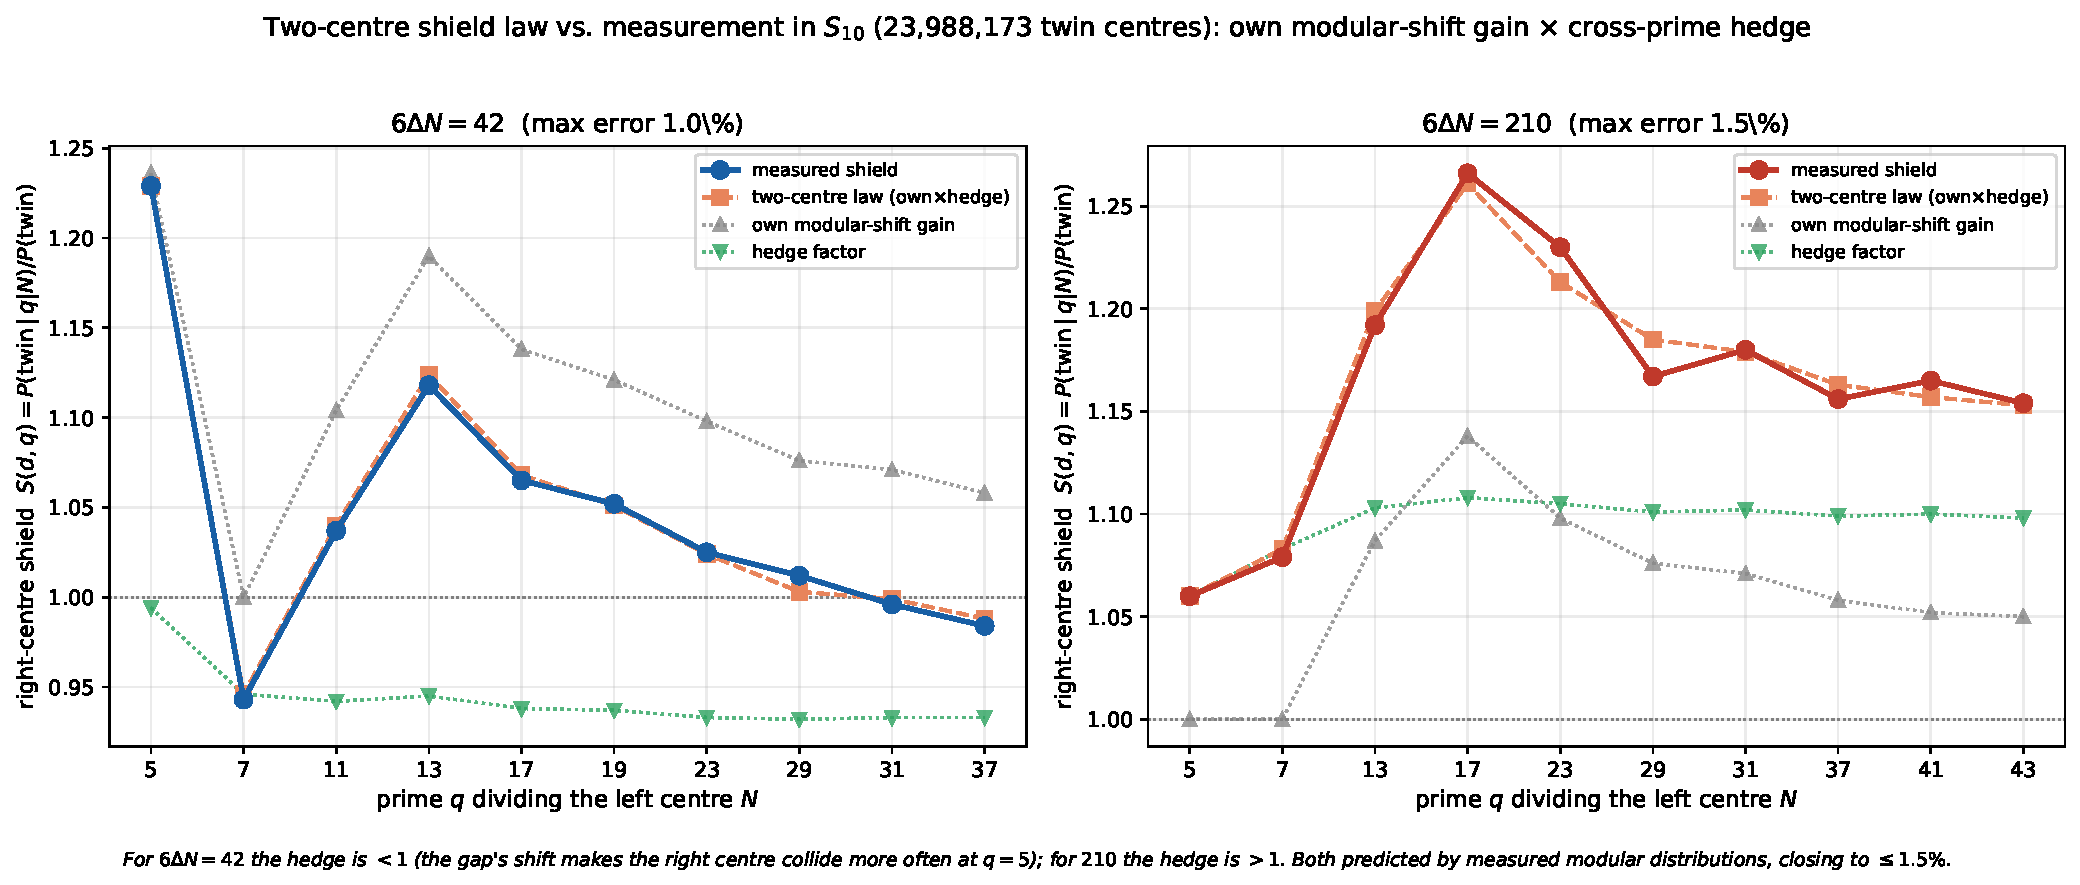
\includegraphics[width=\textwidth]{fig_paper5_twocentre.pdf}
\caption{Measured shield $S(d,q)$ (solid) versus the law $g\times h$ (dashed),
with the two factors shown separately. The gain (grey) and hedge (green) must be
multiplied to match; the hedge is $<1$ for $42$ and $>1$ for $210$.}
\label{fig:tc}
\end{figure}

\begin{table}[h]\centering
\small
\begin{tabular}{rcccc@{\hskip 2em}cccc}
\toprule
& \multicolumn{4}{c}{$6\Delta N=42$} & \multicolumn{4}{c}{$6\Delta N=210$}\\
\cmidrule(lr){2-5}\cmidrule(lr){6-9}
$q$ & gain & hedge & pred. & meas. & gain & hedge & pred. & meas.\\
\midrule
 5 & 1.236 & 0.994 & 1.229 & 1.229 & 1.000 & 1.060 & 1.060 & 1.060\\
 7 & 1.000 & 0.946 & 0.946 & 0.943 & 1.000 & 1.083 & 1.083 & 1.079\\
13 & 1.190 & 0.945 & 1.124 & 1.118 & 1.087 & 1.103 & 1.199 & 1.192\\
17 & 1.138 & 0.938 & 1.068 & 1.065 & 1.138 & 1.108 & 1.261 & 1.266\\
23 & 1.098 & 0.933 & 1.024 & 1.025 & 1.098 & 1.105 & 1.213 & 1.230\\
29 & 1.076 & 0.932 & 1.003 & 1.012 & 1.076 & 1.101 & 1.185 & 1.167\\
31 & 1.071 & 0.933 & 0.999 & 0.996 & 1.071 & 1.102 & 1.179 & 1.180\\
37 & 1.058 & 0.933 & 0.988 & 0.984 & 1.058 & 1.099 & 1.163 & 1.156\\
\bottomrule
\end{tabular}
\caption{Two-centre shield law versus measurement, $S_{10}$. Maximum error
$1.0\%$ ($42$) and $1.5\%$ ($210$). Primes dividing the gap ($7,11,19,41,43$)
are omitted where they lock the gap outright (shield $=0$). The hedge is
systematically $<1$ for $42$ and $>1$ for $210$.}
\label{tab:tc}
\end{table}

The law closes to $\leq1.5\%$ at every admitting prime, for both gaps, and the
same closure holds in $S_9$ (maximum error $3\%$ on a $64\times$ smaller sample).
Two qualitative facts fall out. First, the $42$ shield is a $q=5$ effect: $42$
has $\Delta N=7$, and $N+7\equiv N+2\pmod5$, so $5\mid N$ places the right centre
at the safe residue $2$; the prime $7$ that divides the physical gap is nearly
inert ($g(42,7)=1$). This corrects the natural ``$7\mid42$ is the shield'' guess.
Second, the hedge sign differs by gap: for $42$ the right centre's shift makes it
\emph{more} likely to collide at $5$ (hedge $<1$), for $210$ \emph{less} likely
(hedge $>1$). This is exactly why the single-centre model of Part~IV undershot
$42$ and the absolute survival of $210$ behaved as it did.

\section{What is not yet done: the bridge to the gap distribution}

Proposition~\ref{prop:law} is a law for the \emph{right-centre conditional
survival} given the left centre's factors. It is not yet the gap-preference
$r(d\mid\omega)$ of Part~IV. Passing from one to the other requires summing the
shield over the factor sets that constitute a stratum $\omega$ and integrating
the right-centre survival into a normalised gap distribution---a step we have not
carried out and which need not be a simple average, since the shield depends on
\emph{which} primes divide $N$, not only on how many.

\begin{quote}
\textbf{Open problem.} Bridge the two-centre shield law $S(d,q)=g\,h$ to the
stratified gap preference $r(d\mid\omega)$ of Part~IV, and determine whether it
accounts for the residual high-$\omega$ rise of $42$ (observed $1.55$ at
$\omega=6$ in $S_{10}$). The shield is established at the level of single
conditioning primes and their measured cross-prime hedge; the bridge to the
$\omega$-stratified distribution is open.
\end{quote}

\section{Conclusion}

The two-centre correlation that Parts~II--IV isolated as the missing mechanism is,
at the level of the right-centre conditional survival, a clean and measurable
product of a modular-shift gain and a cross-prime hedge, closing to $\leq1.5\%$
on $2.4\times10^{7}$ twin centres. Both factors are genuinely two-centre and both
require the measured (not idealised) modular distribution of twin centres. The
mechanism overturns two natural guesses---that the gap's own prime factor ($7$
for $42$) is the shield, and that cross-prime effects are negligible---and shows
instead that the shield is a $q=5$ modular-shift effect dressed by a small,
sign-definite hedge. We do not bridge this back to the gap-preference
distribution here; that, and with it the final fate of the $42$ residual, is left
as the open problem. As throughout, no claim is made about the infinitude of twin
primes or any $k$-tuple conjecture; this is a measured, factor-resolved law for
the conditional structure of the $6N$ twin skeleton.

\paragraph{Data and code availability.}
The interferometric scan and the gain/hedge decomposition are openly
available~\cite{repo}; the $S_{10}$ twin count $23{,}988{,}173$ matches Part~I.

\begin{thebibliography}{9}
\bibitem{ChenI} R.~Chen, \emph{Prime distribution on the $6N$ skeleton} (Part~I),
Zenodo, doi:10.5281/zenodo.20470367 (2026).
\bibitem{ChenII} R.~Chen, \emph{Prime gaps on the $6N$ skeleton} (Part~II),
Zenodo, doi:10.5281/zenodo.20477664 (2026).
\bibitem{ChenIII} R.~Chen, \emph{A first-order conditional singular series}
(Part~III), Zenodo, doi:10.5281/zenodo.20498668 (2026).
\bibitem{ChenIV} R.~Chen, \emph{A second-order conditional singular series:
the spatial-compression penalty} (Part~IV), Zenodo, doi:10.5281/zenodo.20500465 (2026).
\bibitem{HL} G.~H.~Hardy, J.~E.~Littlewood, \emph{Partitio Numerorum III}, Acta
Math.\ \textbf{44} (1923), 1--70.
\bibitem{repo} R.~Chen, \emph{$6N$ twin-prime two-centre shield: data and code},
\url{https://github.com/Ruqing1963/6N-twin-prime-two-centre-shield} (2026).
\end{thebibliography}

\end{document}
